\chapter{Einleitung}
\label{Kapitel:Einleitung}

Was ist Buisness Warehouse und Data Warehouse kurze Definition \\
Ein Data Warehouse ist kein Produkt, sondern ein Konzept, das sich der Datenproblematik von managementunterstuetzenden Systemen annimmt\\
A data warehouse is a subject-oriented, integrated, nonvolatile, time-variant collection of data in support of management’s decision \\

1. subject-oriented: Die Themenausrichtung an Sachverhalten des Unternehmens, z.B. Kunden- oder Produktkriterien, wird im BW durch das konsequente Einordnen aller Daten in Fachbereiche und durch die Bezugnahme auf Geschäftsprozesse realisiert (Seemann/Schmalzridt/Lehmann 2001, 18). Im Gegensatz dazu sind operative Daten immer auf einzelne betriebliche Funktionen bezogen (Schinzer/Bange/Mertens 1999, 14 - Bange/ Schinzer o.J., 1). \\
2. integrated: Mit dem DW-Konzept wird eine unternehmensweite Integration von Daten in einem einheitlich gestalteten System angestrebt (Mucksch/Behme 2000, 11). Verein- heitlichung und Integration externer und interner Daten bedeutet weniger die physische Zentralisierung der Daten in einem einzigen Datenpool, sondern deren logische Ver- bindung. Integration bedeutet konsistente Datenhaltung im Sinne einer Struktur- und Formatvereinheitlichung durch Maßnahmen wie Vergabe eindeutiger Bezeichnungen, Anpassung der Datenformate und Herstellung einer semantischen Integrität (Mucksch/ Behme 2000, 11ff.). Ebenso tragen Elemente wie einheitliche Merkmale und standardi- sierte Kennzahlen zu einer Datenintegration bei.\\
3. nonvolatile: Bei einem DW handelt es sich um eine dauerhafte Sammlung von Informationen, auf die im Gegensatz zu OLTP-Systemen (online transaction processing3) nur in Form von Lese- und Einfügeoperationen zugegriffen werden darf, um die Nicht- Volatilität der Daten sicherzustellen.4 Dieser Forderung kann jedoch nur bedingt zuge- stimmt werden, da Korrekturen von aus Quellsystemen geladenen Daten auf jeden Fall möglich sein müssen (Behme 1996, 31). Das BW bietet hierfür eine Eingangsablage in Form der Persistent Staging Area (PSA)5, in der manuelle Korrekturen zur Validierung und Fehlerbehebung nach dem Extraktionsvorgang durchgeführt werden können (SAP 2000a, 1; SAP 2000b).\\
4. time-variant: Während bei operativen Systemen eine zeitpunktgenaue Betrachtung der Daten im Mittelpunkt steht, liegt das Interesse bei Auswertungen im DW eher in einer Zeitraumbetrachtung, z.B. einer Trendanalyse (Behme 1996, 31). Der Zeitraumbezug ist daher impliziter oder expliziter Bestandteil der Daten in einem DW. Ein Ansatz zur Herstellung dieses Zeitraumbezugs im BW ist die obligatorische Verwendung einer Zeitdimension in jedem Informationsspeicher.


\begin{figure}[H]
    \centering
    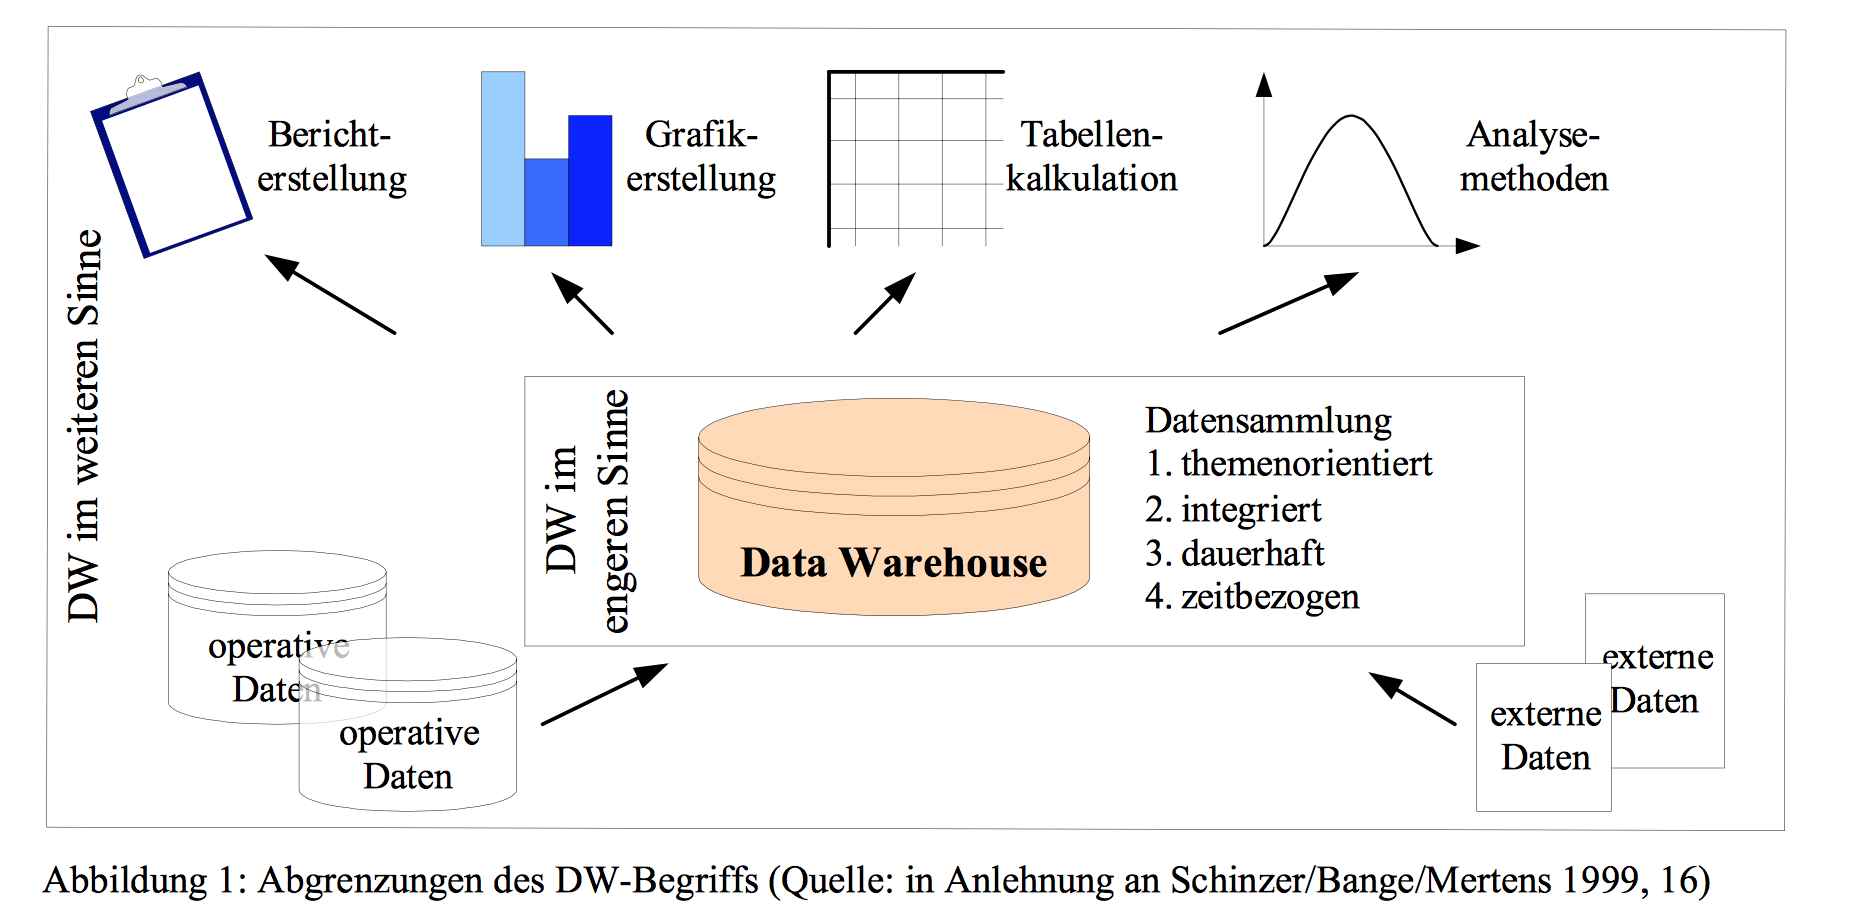
\includegraphics[width=.8\textwidth]{files/DWOverview}
    \caption{unterschrift}
    \label{pic:DWOverview}
\end{figure}



\section{Unterkapitel}
\label{Abschnitt:Motivation}


Text
